\setchapterpreamble[u]{\margintoc}
\chapter{Introduzione}

\begin{chap-intro}
Relazione relativa al progetto d'esame \enquote{\textbf{FruitNinjaGL} (fnGL)} del corso di Computer Grahics: Animation and Simulation (GraficInt, aa 2019)
\end{chap-intro}

\section{Introduzione}
\begin{marginfigure}
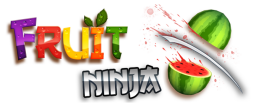
\includegraphics[width=\linewidth]{images/ch10/0}
\caption{Logo di Fruit Ninja}
\end{marginfigure}
L'applicativo sviluppato come progetto d'esame è un clone in OpenGL del famossissimo \textbf{Fruit Ninja} videogioco sviluppato dalla \textit{Halfbrick Studios} e pubblicato nel 2010 per sistemi iOS ed Android diventando rapidamente una delle applicazioni più scaricate; Ad oggi il numero totale di download supera il miliardo.

Il gioco è stato riproposto in molteplici versioni e piattaforme tra le principali abbiamo \textbf{Fruit Ninja Kinect} per Xbox e Windows, \textbf{Fruit Ninja THD} ottimizzato per dispositivi con Nvidia Tegra 2, \textbf{Fruit Ninja VR} per Oculus, HTC Vive e PlayStation 4 ed infine un arcade game chiamato \textbf{Fruit Ninja FX}.


\subsection{Gameplay}
In Fruit Ninja il giocatore deve affettare della frutta che viene lanciata sullo schermo, trascinando un dito sul touch screen del dispositivo. Lo scopo del gioco è quello di tagliare più frutta possibile. Vengono conferiti punti extra quando si affettano tre o più frutti con uno stesso swipe chiamate \textit{combo}, anche l'esecuzione ripetuta di combo chiamata \textit{blitz} conferisce punti aggiuntivi.

\begin{figure}[!htp]
	\centering
	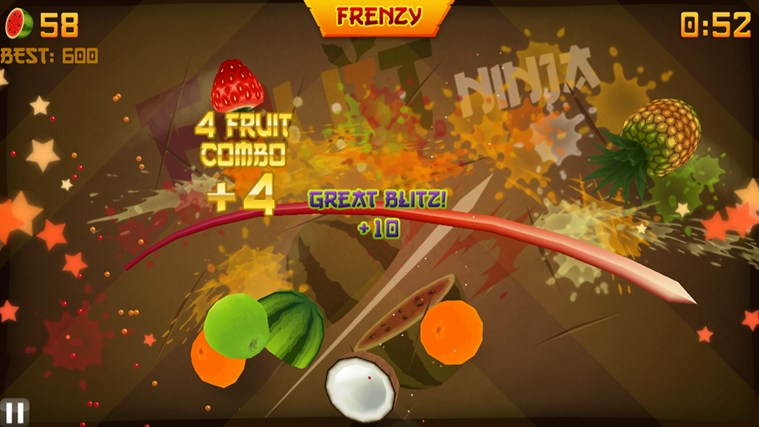
\includegraphics[width=0.49\linewidth]{images/ch10/4} \hfill
	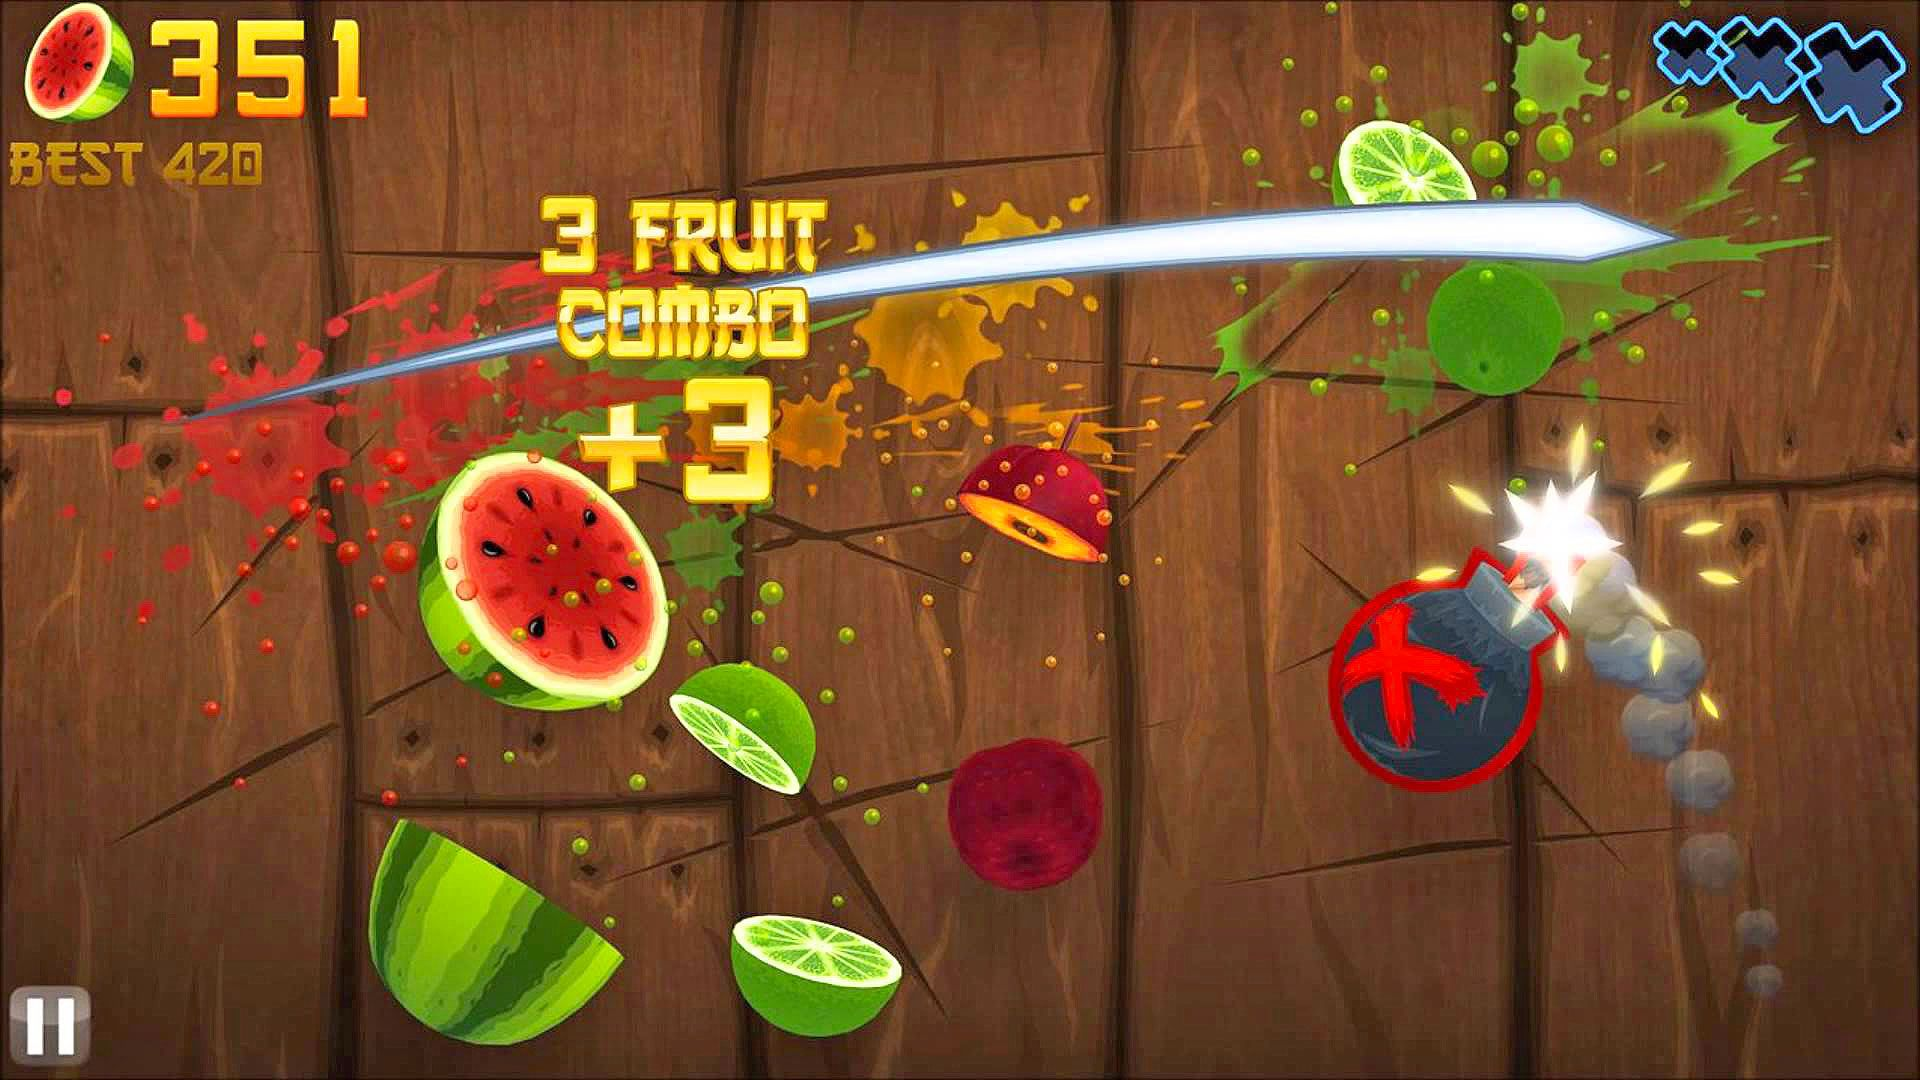
\includegraphics[width=0.49\linewidth]{images/ch10/1}
	\\[0.15cm]
	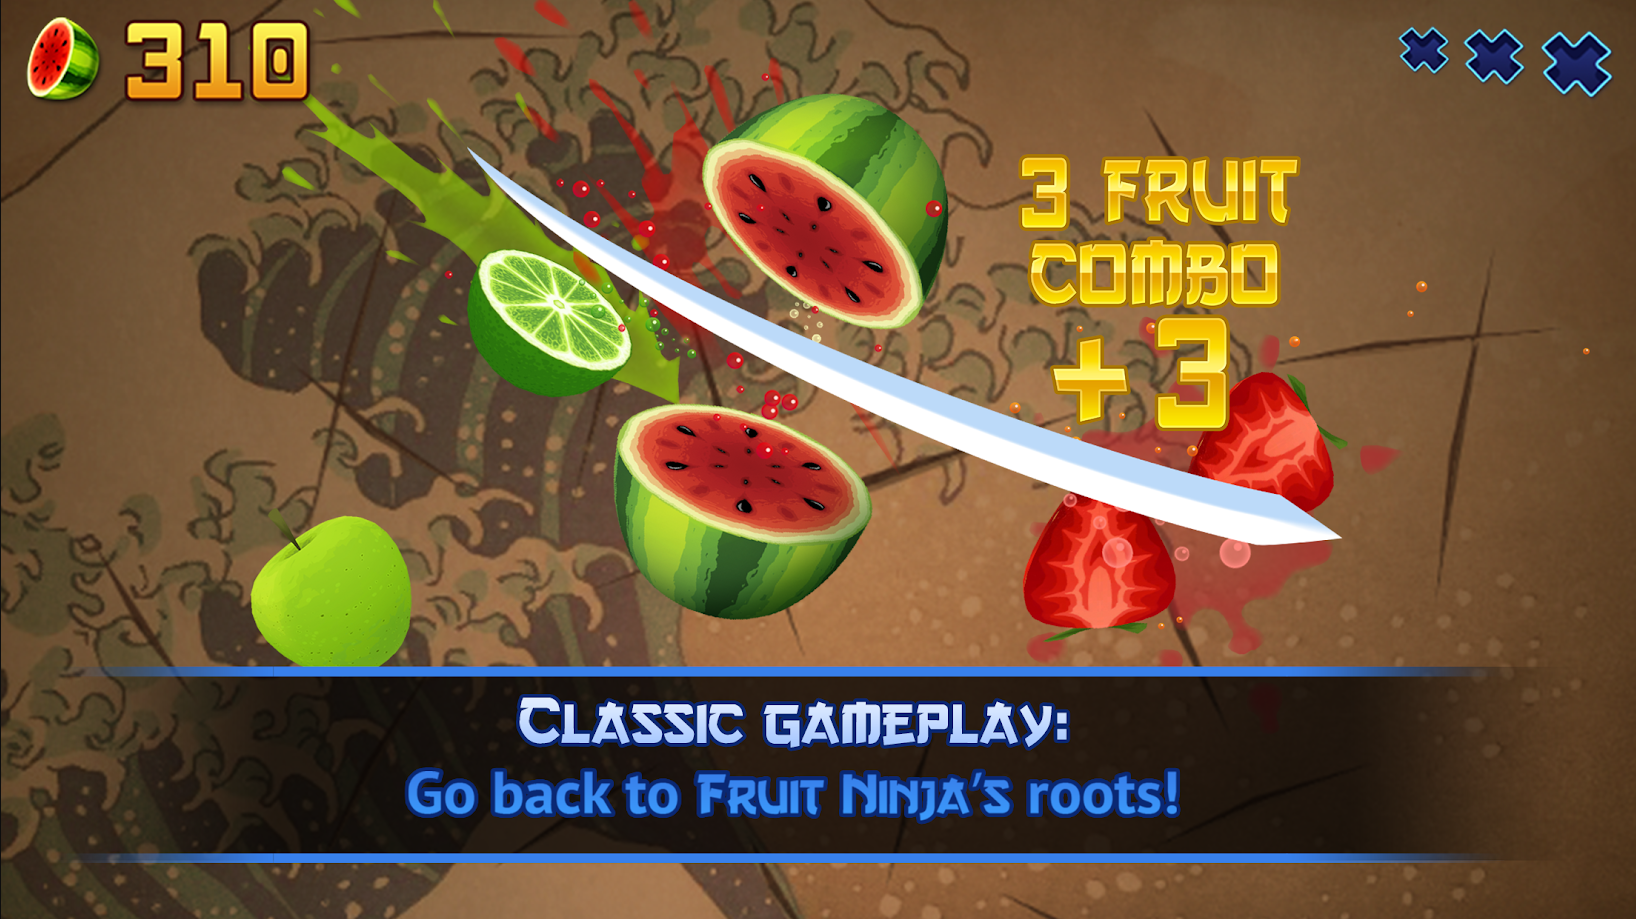
\includegraphics[width=0.49\linewidth]{images/ch10/2} \hfill
	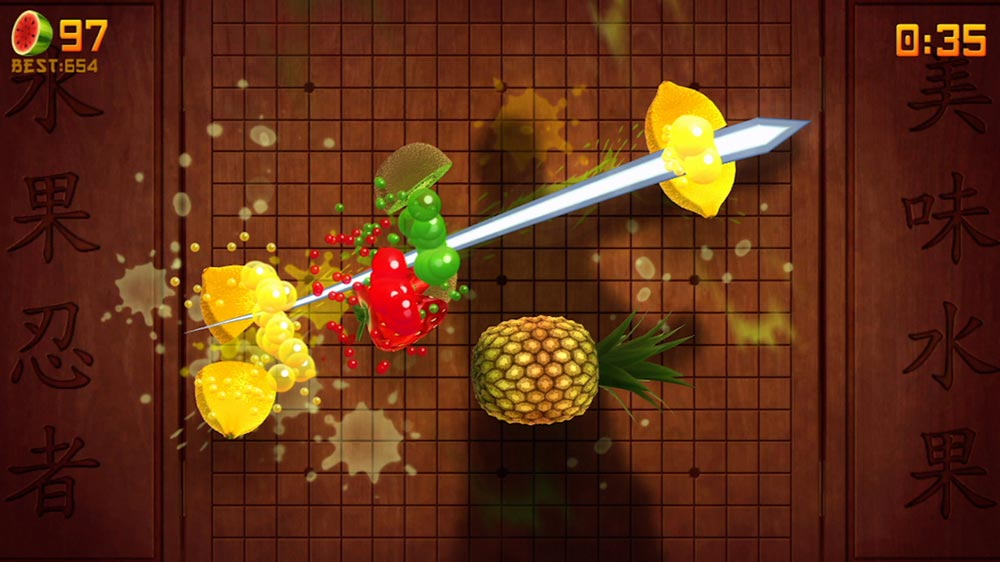
\includegraphics[width=0.49\linewidth]{images/ch10/3}	
	
	\caption{Esempio di alcune versioni e modalità di gioco di Fruit Ninja. Da sinistra verso destra abbiamo (1) Screen della prima versione originale, (2) Versione HD, (3) Ultima versione con un ritorno al passato, (4) Versione VR. }
\end{figure}

Fruit Ninja mette a disposizione diverse modalità di gioco che si basano tutte sul gameplay appena descritto:
\begin{itemize}
\item \textbf{Classica}: Il giocatore ha a disposizione tempo illimitato e 3 vite, insieme ai frutti possono essere lanciate anche delle bombe esplosive da evitare. Ogni frutto mancato causa la perdita di una vita, se si colpisce una bomba oppure si perdono tutte le vite il gioco terminerà. Ogni cento punti si guadagna una vita. Non ci sono limiti alla durata della partita o del punteggio se non la bravura del giocatore.
\item \textbf{Arcade}: Dura 60 secondi, l'obiettivo è battere il record. Le differenze dalla modalità classica sono: il tempo è limitato, non vi sono vite\sidenote{la frutta mancata non causa effetti negativi.} e per ogni bomba colpita il tempo rimasto viene diminuito di 10 secondi. Sono inoltre presenti banane speciali con effetti speciali che conferiscono brevi bonus quando tagliate.
\item \textbf{Zen}: Nella modalità Zen, la durata della partita è di 1:30 minuti l'obiettivo è battere il record, non saranno presenti bombe e vite e si dovrà quindi unicamente cercare di affettare più frutta possibile puntando sulle combo senza l'ausilio di bonus. 
\end{itemize}
Per lo sviluppo del progetto si è scelta come base la \textbf{modalità Zen}.





\section{Fruit Ninja GL}
\begin{marginfigure}
	
\includegraphics[width=\linewidth]{images/ch10/6}
	\caption{Logo della software di fantasia che ha sviluppato il fnGL.}
\end{marginfigure}
In questa relazione verrà descritto \textbf{Fruit Ninja GL} (da ora in poi abbreviato con \textbf{fnGL}) clone sviluppato in OpenGL dalla \textbf{\textit{Space Mambo Studios}} un'immaginaria software house. L'idea di base è quella di replicare la modalità Zen del gioco integrandola però di alcune caratteristiche mancanti\sidenote[*+2][]{Nel gioco originale, mancano totalmente Luci e Collisioni tra i frutti i quali semplicemente si sovrappongono.} ma necessarie ai requisiti del progetto senza però snaturare o alterare il gameplay originale.

\begin{figure}[!htp]
	\centering
	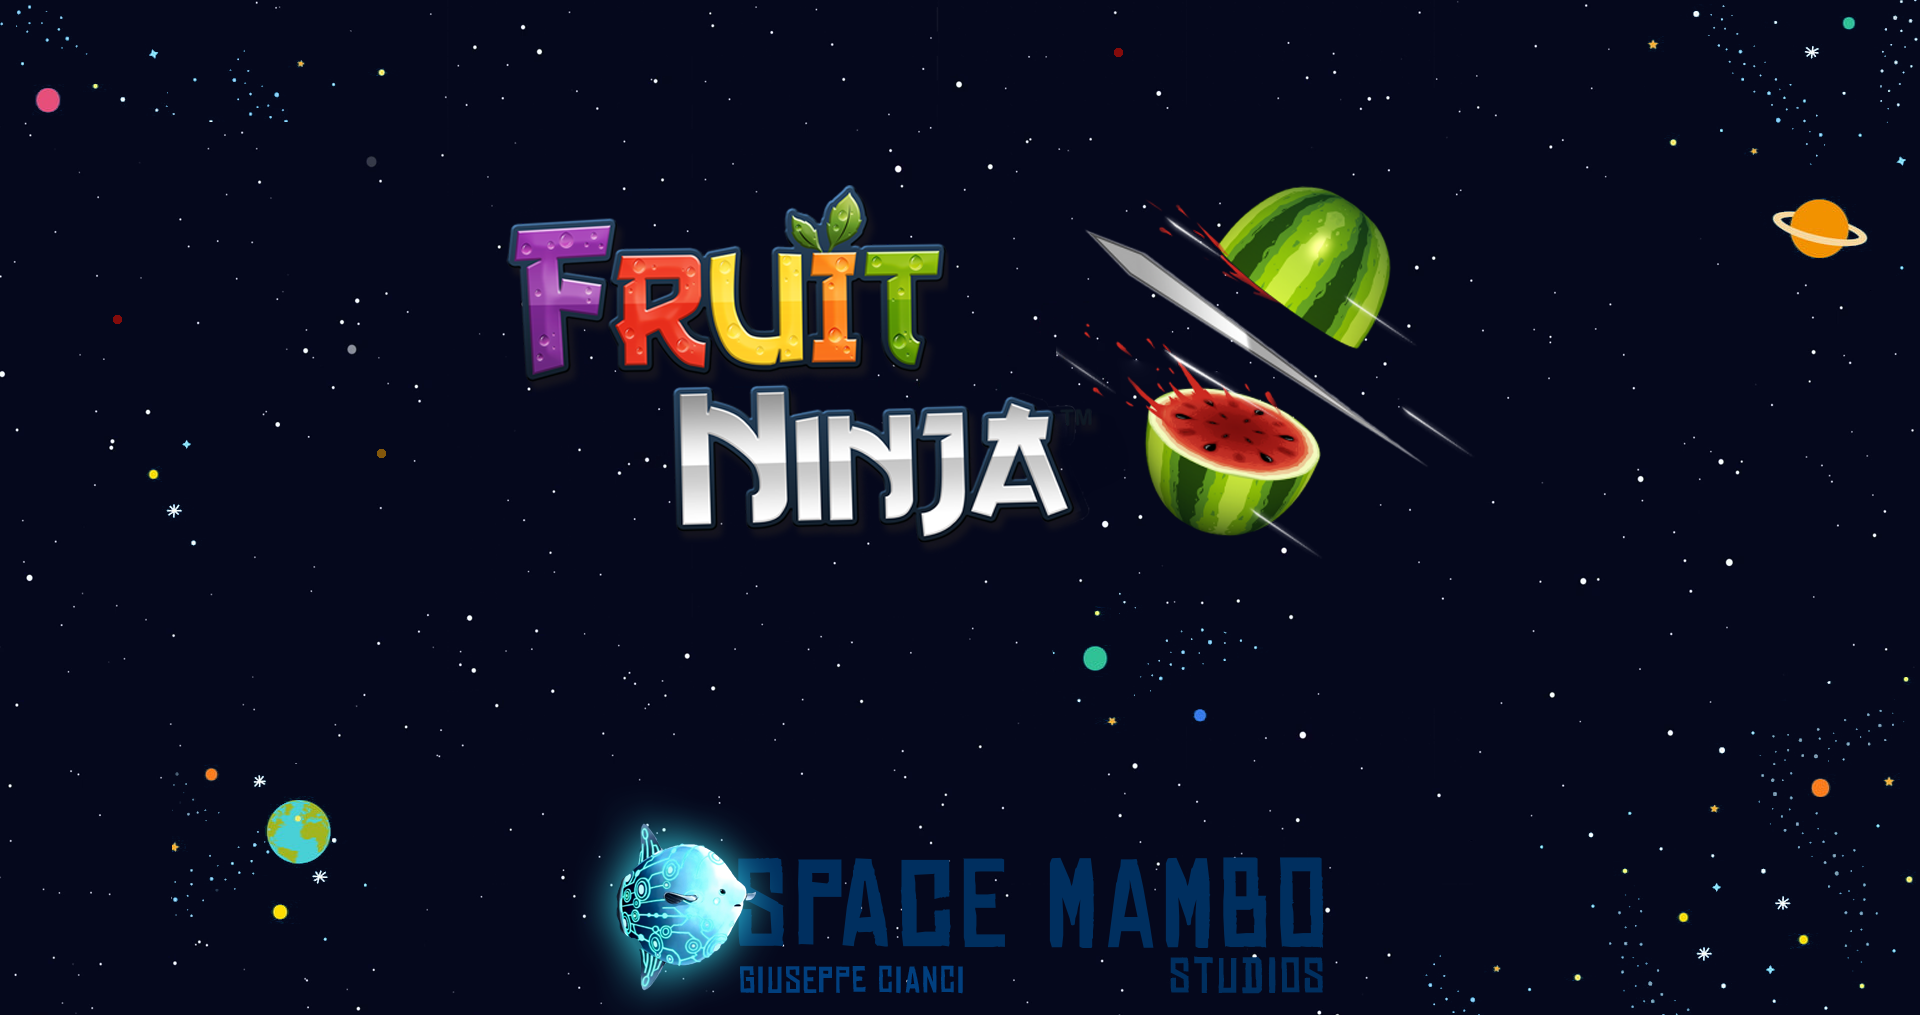
\includegraphics[width=0.49\linewidth]{images/ch10/a2} \hfill
	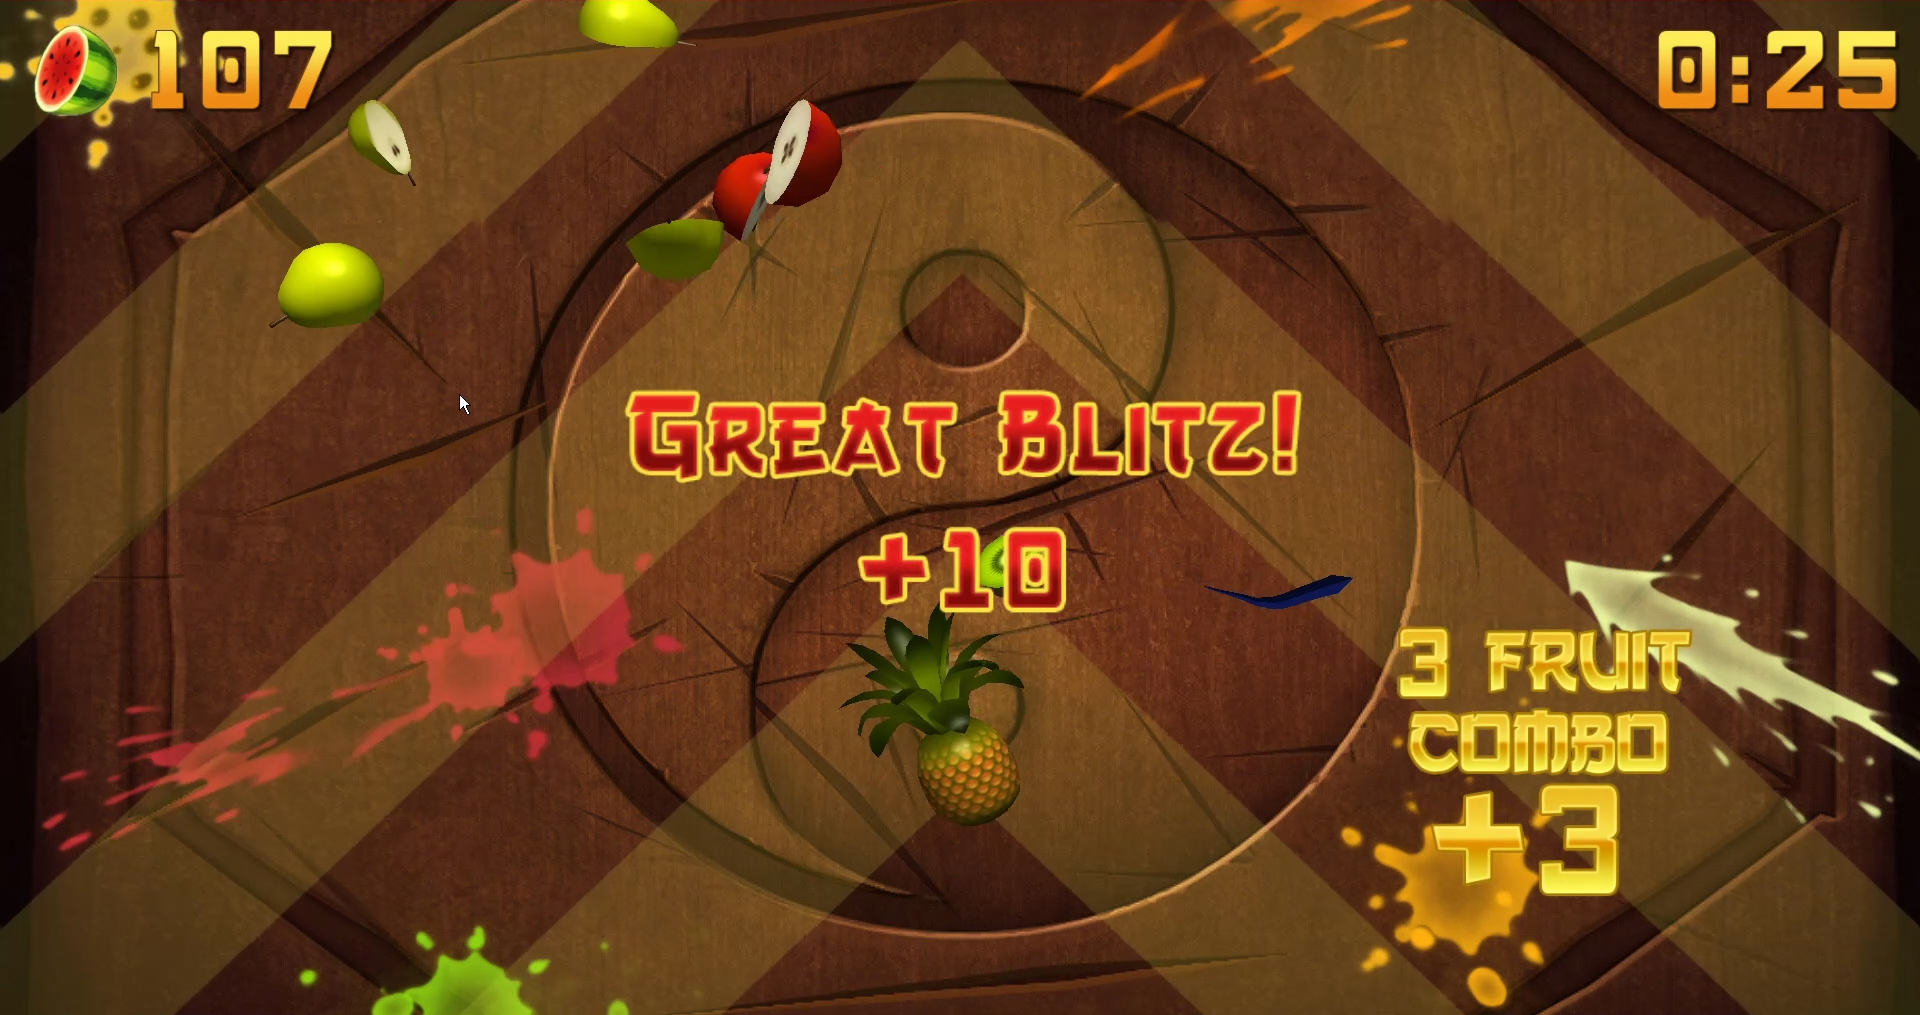
\includegraphics[width=0.49\linewidth]{images/ch10/a1}
	\\[0.15cm]
	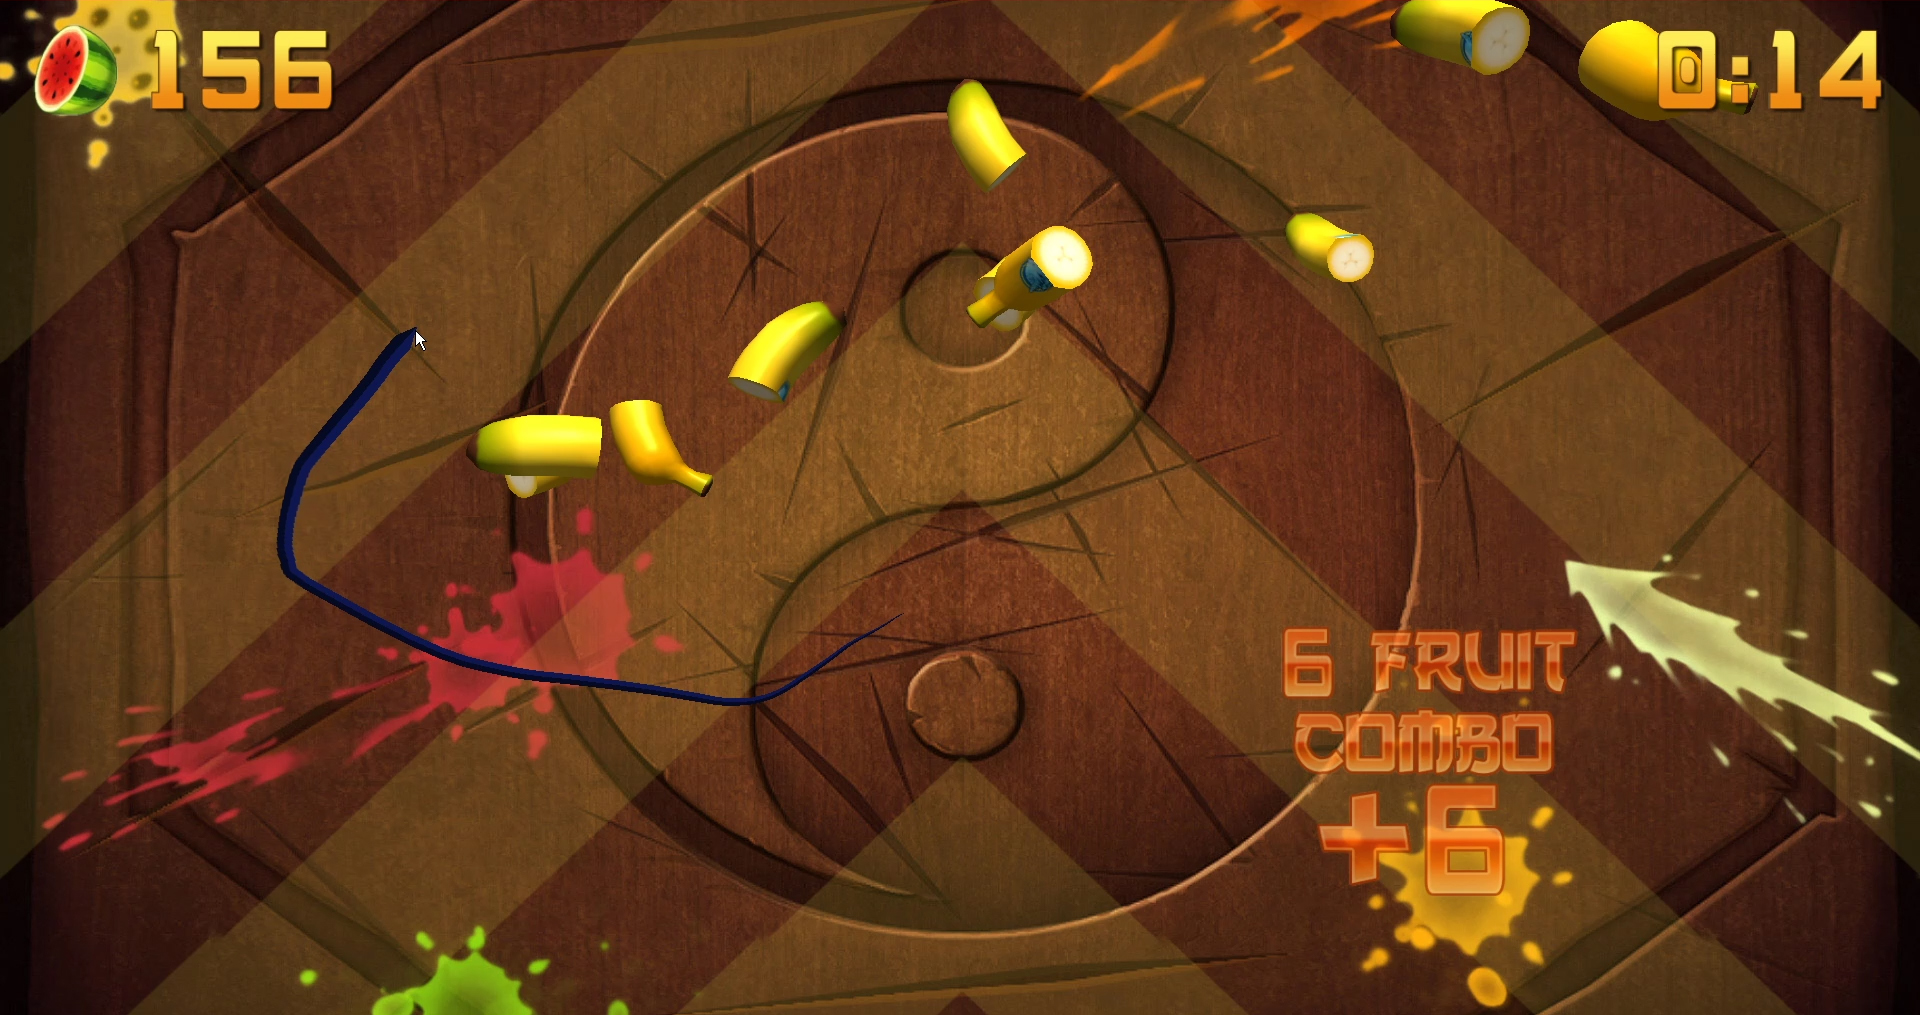
\includegraphics[width=0.49\linewidth]{images/ch10/a3} \hfill
	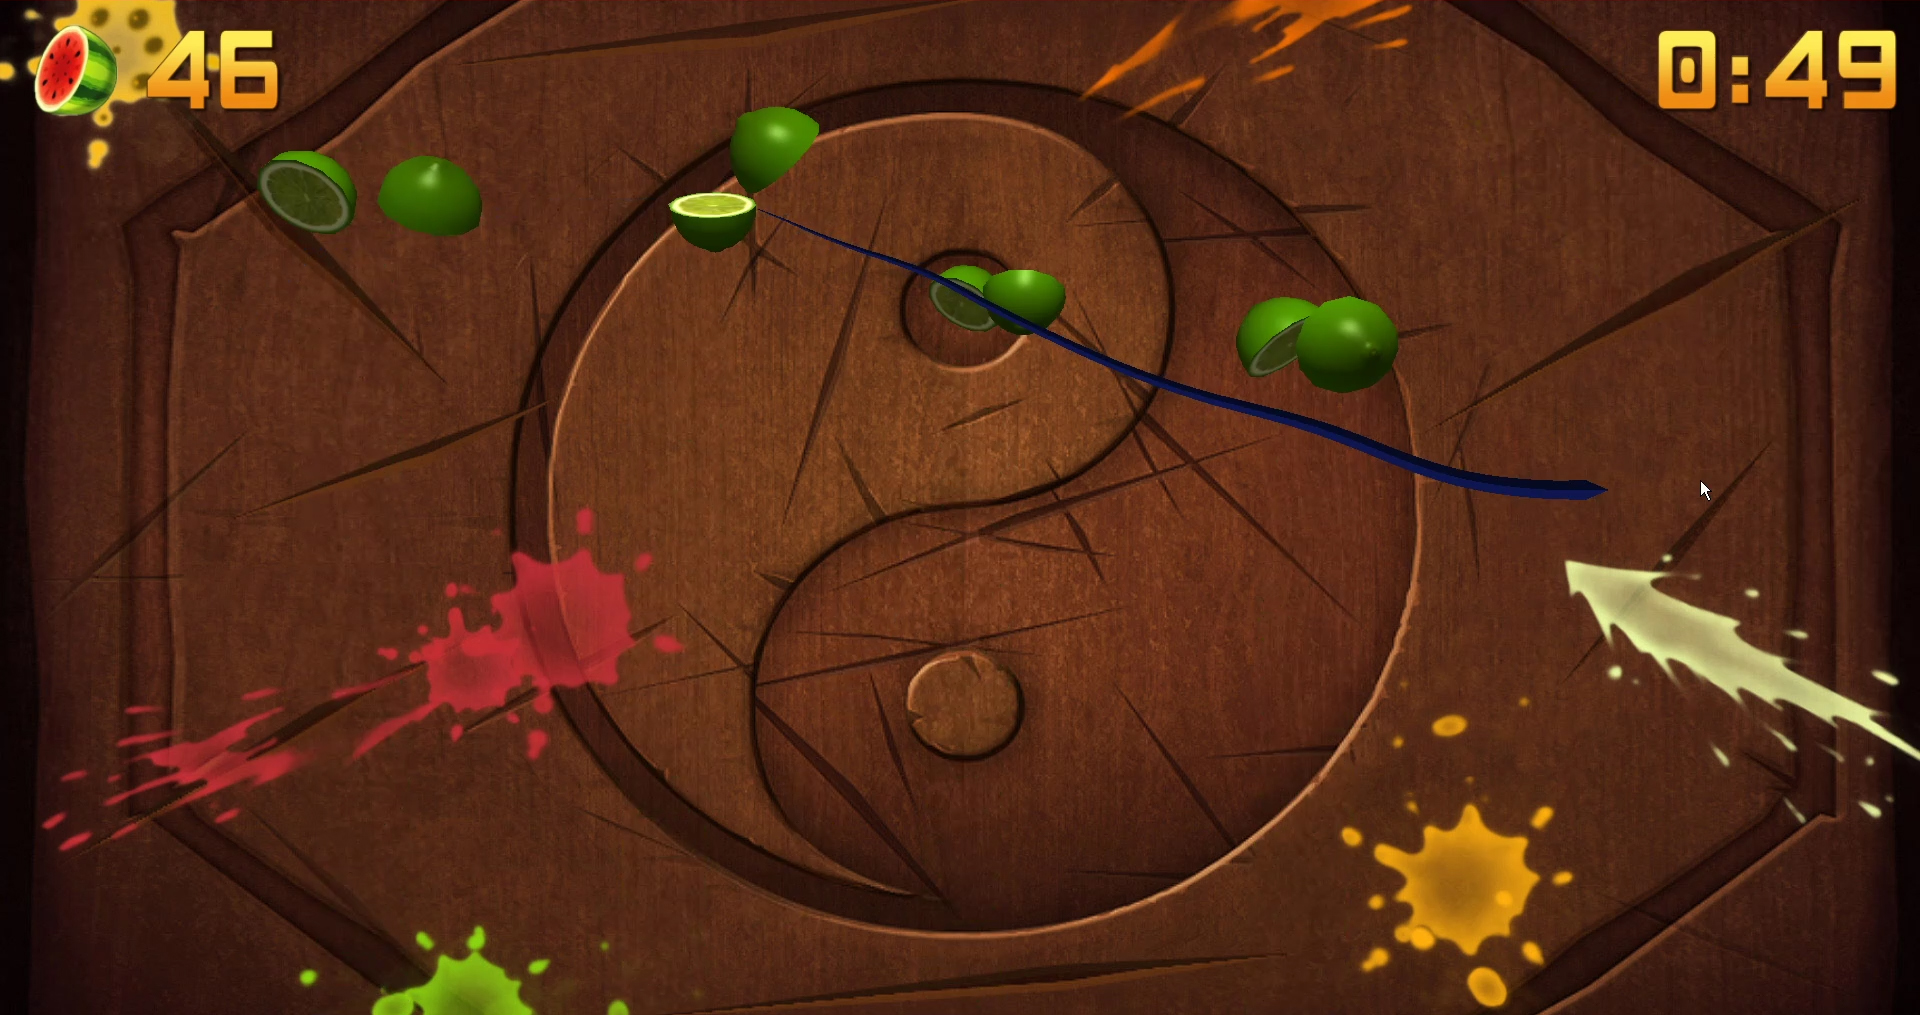
\includegraphics[width=0.49\linewidth]{images/ch10/a4}	
	
	\caption{Alcuni screen di gioco di Fruit Ninja GL.}
\end{figure}

Il giocatore avrà a disposizione 1:30 minuti per affettare quanti più punti possibili effettuando \textit{combo} e \textit{blitz} per massimizzare il punteggio finale. A completare il tutto sono presenti le musiche e gli effetti originali del gioco cercando di replicare nel dettaglio anche la grafica.

\subsection{Librerie e Software Utilizzati}
Fruit Ninja GL è stato sviluppato utilizzando C++20 in ambiente Visual Studio ed è basato sull'ultima versione disponibile di OpenGL la 4.6; Oltre a ciò sono state impiegate diverse librerie o moduli per semplificare lo sviluppo del gioco:
\begin{itemize}
\item \texttt{GLFW} \cite{GLFW}: Libreria open-source, multi-piattaforma per OpenGL. Fornisce una semplice API per la creazione di finestre, contexts e la gestione di diverse tipologie input ed eventi.

\item \texttt{GLEW} \cite{GLEW}: Libreria multi-piattaforma open-source per il loading delle funzioni OpenGL. Fornisce un meccanismo moderno ed efficiente per determinare, a run-time, quale estensione di OpenGL è supportata dalla piattaforma target. 

\item \texttt{GLM} \cite{GLM}: Libreria matematica basata sulle specifiche\sidenote{Le funzionalità non sono però limitate al GLSL ma si estendono anche alle trasformazioni matriciali, quaternioni, data packing, random numbers, noise, etc...} del OpenGL Shading Language (GLSL). 

\item \texttt{ASSIMP} \cite{ASSIMP}: Libreria open-source che fornisce una API semplice ed unificata per la gestione di vari formati di modelli 3D, in particolare consentendone il caricamento, lattura oltre che l'esportazione. 

\item \texttt{stb\_image} \cite{STB}: Libreria open-source che consente il loading/decoding da file o memoria di immagini nei formati più comuni.

\item \texttt{irrKlang} \cite{IRRKLANG}: Libreria ad alto livello che consente il caricamento e l'esecuzione di numerosissimi formati audio.

\item \texttt{\{fmt\}} \cite{FMT}: Libreria open-source per il format delle stringhe. 

\item \texttt{ImGUI} \cite{IMGUI}: Libreria per il disegno di GUI interattive \sidenote{Utilizzata nelle fasi iniziali di sviluppo più per un rapido debug e prototipazione. Rimossa nelle fasi finali del progetto.}. 
\end{itemize} 

Inoltre è stato utilizzato \textbf{Visual Studio 2019} per lo sviluppo, \textbf{Adobe Photoshop} per la creazione di sprite e l'editing di texture ed in fine \textbf{Doxygen} + \textbf{m.css}\footnote{A modern, mobile friendly drop-in replacement for the stock Doxygen HTML output. \url{https://mcss.mosra.cz/mcss/documentation/doxygen/}} per la produzione della documentazione.


\subsection{Documentazione}
Tutto il codice è ben documentato e correlato di una documentazione prodotta dai commenti che descrive i vari moduli, classi e funzioni implementati.

\begin{figure}[!htp]
	\centering
	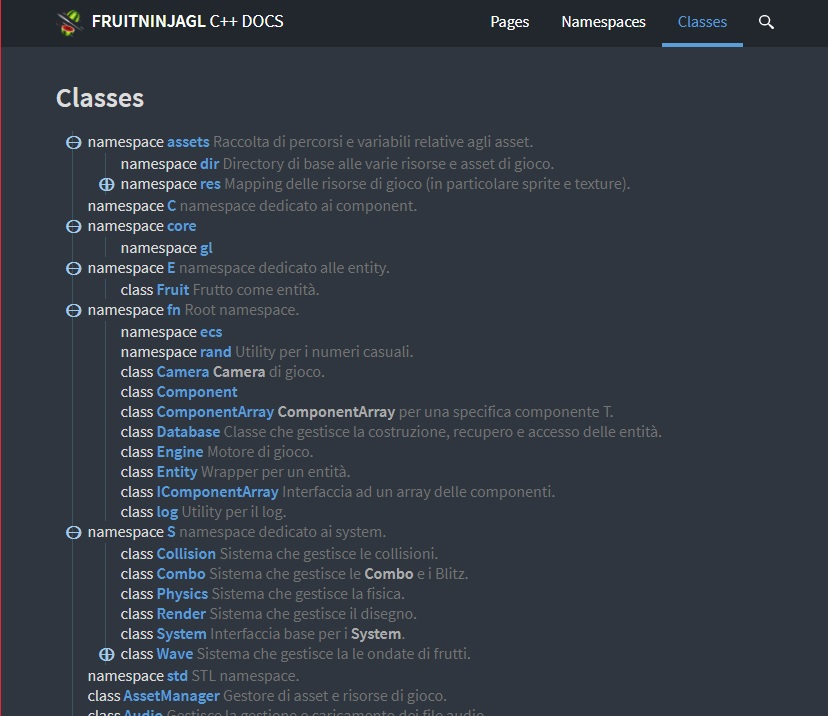
\includegraphics[width=0.9\linewidth]{images/ch10/5}
	\caption{Esempio della documentazione prodotta con Doxygen + m.css. Nella figura è mostrata la lista della classi. }
\end{figure}




\subsection{Avvio dell'applicazione}
Per poter avviare l'applicazione è necessario effettuare una sorta di processo di installazione\sidenote{L'ultima versione dell'eseguibile è già stata spostata ed è attualmente presente.}.

Una volta compilata l'applicazione l'eseguibile generato va spostato all'{}interno della cartella \texttt{./FruitNinjaGL/FruitNinjaGL/} ovvero quella dove sono presenti i file di progetto VisualStudio; Tale operazione è fondamentale per accedere ai file \texttt{.dll} per il linking delle librerie e alla cartella \texttt{./res} contenente tutti gli asset e risorse di gioco i cui percorsi sono relativi alla workspace del progetto.





















































%
















